\chapter{Experiment}

\section{Experimental Setup}

\subsection{Data Split and Target}
We use a strict chronological split to avoid look-ahead bias:
\begin{itemize}
	\item Training years: 2019--2023
	\item Validation year: 2024
	\item Test year: 2025
\end{itemize}

The prediction target is 5-day ahead return \texttt{future\_ret\_5}.

\subsection{Input Features}
All models are trained on the same 15 engineered price/fundamental features to ensure fair comparison:
\begin{align*}
\{&\texttt{ret\_1},\texttt{ret\_5},\texttt{ret\_10},\texttt{ret\_20},\texttt{hl\_spread},\texttt{co\_ret},\texttt{log\_vol},\\
&\texttt{turnover\_rate},\texttt{volume\_ratio},\texttt{pb},\texttt{ma5\_gap},\texttt{ma10\_gap},\texttt{ma20\_gap},\\
&\texttt{volatility\_5},\texttt{volatility\_20}\}
\end{align*}

For sequence models (LSTM/GRU), the sequence length is 30 and features are normalized per sequence by max-abs scaling.

\subsection{Baselines and Metrics}
We evaluate five non-graph baselines:
\begin{itemize}
	\item Linear factor model: Ridge
	\item Nonlinear tabular models: LightGBM, XGBoost
	\item Deep temporal models: LSTM, GRU
\end{itemize}

Reported metrics include IC, RankIC, SignAcc, Sharpe, MSE, and cross-sectional Top-$k$ portfolio metrics (IRR/Sharpe).

\section{Main Results}

\begin{table}[htbp]
\centering
\caption{Test-set performance comparison (2025)}
\label{tab:main-test-results}
\begin{tabular}{lccc}
\hline
Model & Test IC & Test RankIC & Top10 Sharpe \\
\hline
Ridge & 0.03568435 & 0.00069723 & -- \\
LightGBM & 0.04974221 & 0.01374122 & 4.37949639 \\
XGBoost & 0.04866105 & 0.01128825 & 4.55806821 \\
LSTM & 0.02906183 & 0.02642975 & 2.55264244 \\
GRU & \textbf{0.05160307} & \textbf{0.04237023} & 4.41701568 \\
\hline
\end{tabular}
\end{table}

The results show two clear findings:
\begin{itemize}
	\item The 15 engineered price factors carry meaningful predictive signal across all model families.
	\item GRU and tree models form very strong non-graph baselines; GRU achieves the highest test IC, while XGBoost achieves the highest Top10 Sharpe.
\end{itemize}

\section{Model-by-Model Analysis}

\subsection{Tree Models: Strong and Stable}
Both LightGBM and XGBoost remain highly competitive:
\begin{itemize}
	\item LightGBM: Test IC $=0.04974221$, Top10 Sharpe $=4.3795$
	\item XGBoost: Test IC $=0.04866105$, Top10 Sharpe $=4.5581$
\end{itemize}
These two models are strong tabular baselines for the final comparison table.

\subsection{GRU: Best IC in This Round}
GRU delivers the strongest test IC among all five models:
\begin{itemize}
	\item Test IC $=0.05160307$
	\item Test RankIC $=0.04237023$
	\item Top10 Sharpe $=4.4170$
\end{itemize}
Therefore, under the current single-modality price-factor setting, GRU is at least on par with tree models and slightly better in IC.

\subsection{LSTM: Usable but Unstable}
LSTM is not completely ineffective, but it is unstable during training:
\begin{itemize}
	\item Best epoch appears at epoch 1
	\item Best validation IC $=0.05708638$
	\item Test IC $=0.02906183$
\end{itemize}
This suggests LSTM can capture some signal but quickly loses generalization after further optimization. In this task, GRU is better aligned than LSTM.

\subsection{Ridge: Important Linear Reference}
Ridge reaches Test IC $=0.03568435$, lower than nonlinear models but still clearly positive. This provides a robust linear multi-factor baseline and supports the value of nonlinear methods.

\section{Short-Horizon Target: Why \texttt{ret\_1} Looks Easier}

In a supplementary run, we also replace the 5-day return target with the 1-day return target \texttt{future\_ret\_1}. The main empirical observation is that the IC becomes higher, but this does not mean the model becomes fundamentally stronger. The prediction task itself is easier.

\subsection{Microstructure Effects Matter More at One Day}

One-day returns are more sensitive to local market microstructure, such as intraday sentiment, liquidity pressure, and order flow. These effects are easier for our engineered features to capture, especially volume-related variables and short-horizon price momentum. As a result, \texttt{ret\_1} is naturally more predictable than \texttt{ret\_5}.

\subsection{Longer Horizons Contain More Noise}

Five-day returns mix in more sources of uncertainty, including macro shocks, sector rotation, and random cross-sectional drift. This increases the noise level of the target. By contrast, one-day returns stay more local and more directly linked to the latest market state, so IC is easier to obtain.

\subsection{Higher IC Does Not Mean Less Overfitting}

The higher \texttt{ret\_1} IC should also be interpreted carefully. A model can achieve a better IC on a simpler short-horizon target while still overfitting short-term patterns. In practice, this is exactly what we observe: train IC remains much higher than validation and test IC, which means the model is still learning short-range structure rather than a fully robust alpha signal.

\subsection{Practical Implication}

This supplementary result is useful because it confirms that the feature set does contain short-horizon predictive information. However, the more important and harder setting is still \texttt{future\_ret\_5}, since it is closer to a realistic portfolio construction horizon and exposes whether the model can generalize beyond local market inertia.

For a concrete reference, the LightGBM run on \texttt{future\_ret\_1} with price and news features gives much stronger in-sample fit than the 5-day target, but the out-of-sample advantage is much smaller:
\begin{itemize}
\item Train IC $=0.29256246$, Val IC $=0.07432835$, Test IC $=0.06360294$
\item Train RankIC $=0.20117949$, Val RankIC $=0.03790694$, Test RankIC $=0.01461429$
\item Train Top10 Sharpe $=15.97407609$, Val Top10 Sharpe $=3.54472250$, Test Top10 Sharpe $=3.89395440$
\item Train Top30 Sharpe $=12.67766503$, Val Top30 Sharpe $=1.94790793$, Test Top30 Sharpe $=3.28545027$
\item Train Top50 Sharpe $=10.57799773$, Val Top50 Sharpe $=1.48605285$, Test Top50 Sharpe $=2.71897655$
\end{itemize}

This pattern is consistent with the previous explanation: \texttt{ret\_1} is easier to fit because it is more local and more sensitive to short-term microstructure, but it also makes overfitting more obvious. The gap between train IC and test IC is still large, so the higher score should be interpreted as a task simplification effect rather than a fundamentally more powerful model.

\section{Generalization Gap and Overfitting}

A noticeable train--validation/test gap remains. For example:
\begin{itemize}
	\item GRU: Train IC $=0.2479$, Val IC $=0.0203$, Test IC $=0.0516$
	\item LightGBM: Train IC $=0.3044$, Val IC $=0.0529$, Test IC $=0.0497$
\end{itemize}
This is consistent with the high-noise nature of short-horizon return prediction in equities. The gap should be acknowledged as a key limitation, but the positive out-of-sample IC confirms that useful signal still exists.

\section{Effect of News Features}

\subsection{Motivation: Why Supplement Price with News?}

Price-based factors capture historical market dynamics but fail to incorporate external information such as news events, which may affect short-term price movements. To assess whether news provides incremental predictive value and to understand how different model architectures utilize such event-driven information, we construct a multimodal experimental setup by augmenting the 15 price factors with 13 daily aggregated news features (28 in total).

The studied models are:
\begin{itemize}
\item LightGBM + price + news
\item XGBoost + price + news
\item GRU + price + news
\end{itemize}

We maintain the same chronological split (train 2019--2023, validation 2024, test 2025) and target \texttt{future\_ret\_5} as the price-only baseline to enable fair comparison.

\subsection{News Feature Construction}

Each raw news item is first scored by sentiment analysis, then aggregated by stock-date. The final news feature set includes:

\begin{itemize}
\item \textbf{Count features:} \texttt{news\_cnt\_1d}, \texttt{news\_cnt\_3d}, \texttt{news\_cnt\_7d}
\item \textbf{Sentiment features:} \texttt{news\_sent\_mean\_1d}, \texttt{news\_sent\_mean\_3d}, \texttt{news\_sent\_mean\_7d}
\item \textbf{Dispersion/extreme features:} \texttt{news\_sent\_std\_7d}, \texttt{news\_sent\_max\_3d}, \texttt{news\_sent\_min\_3d}
\item \textbf{Event polarity/risk features:} \texttt{news\_pos\_cnt\_3d}, \texttt{news\_neg\_cnt\_3d}, \texttt{news\_risk\_cnt\_7d}
\item \textbf{Recency indicator:} \texttt{days\_since\_last\_news}
\end{itemize}

To avoid look-ahead bias, all aggregated news features are shifted by one trading day before being used for prediction. This ensures that only information available at time $t$ is used to predict future returns at time $t+5$.

\subsection{Impact on Tree-Based Models}

Incorporating news features leads to consistent improvements in tree-based models. Table~\ref{tab:news-test-results} shows that LightGBM achieves the best overall performance, with modest gains in IC and more significant improvements in top-$k$ portfolio Sharpe ratios (Table~\ref{tab:news-vs-price-delta}).

The improvement is more pronounced in top-$k$ selection (e.g., Top30 and Top50), where LightGBM gains $\Delta$ Top30 Sharpe $= +0.6213$ and $\Delta$ Top50 Sharpe $= +0.3721$. In contrast, test IC improves by only $\Delta$ IC $= +0.00142$. XGBoost shows a similar pattern: nearly flat IC change ($+0.00008107$) but larger top-$k$ Sharpe gains. 

This indicates that news signals act as a \textbf{filtering mechanism that enhances stock selection} rather than a dominant predictive factor for overall ranking. Tree models can effectively combine price features and news signals to identify higher-conviction investment opportunities.

\subsection{Impact on Sequential Models}

In contrast, incorporating news features into the GRU model results in a noticeable performance degradation (Table~\ref{tab:news-vs-price-delta}). Test IC decreases by $\Delta$ IC $= -0.02468536$, and top-$k$ Sharpe ratios also decline significantly ($\Delta$ Top30 Sharpe $= -0.7100$). The model exhibits early overfitting and fails to generalize to the test set.

This suggests that the current representation of news features is fundamentally unsuitable for sequential modeling. Unlike price features, which exhibit smooth temporal dependencies, news signals are \textbf{sparse, event-driven, and irregular over time}. When concatenated as dense time series inputs, they introduce noise and hinder the learning of temporal patterns inherent to sequential models like GRU.

\subsection{Feature Importance Analysis}

To understand which features contribute most to predictions, we analyze feature importance in the LightGBM model. Figures~\ref{fig:importance-price-only} and~\ref{fig:importance-news-augmented} present the feature importance distributions for price-only and news-augmented LightGBM respectively.

\begin{figure}[htbp]
\centering
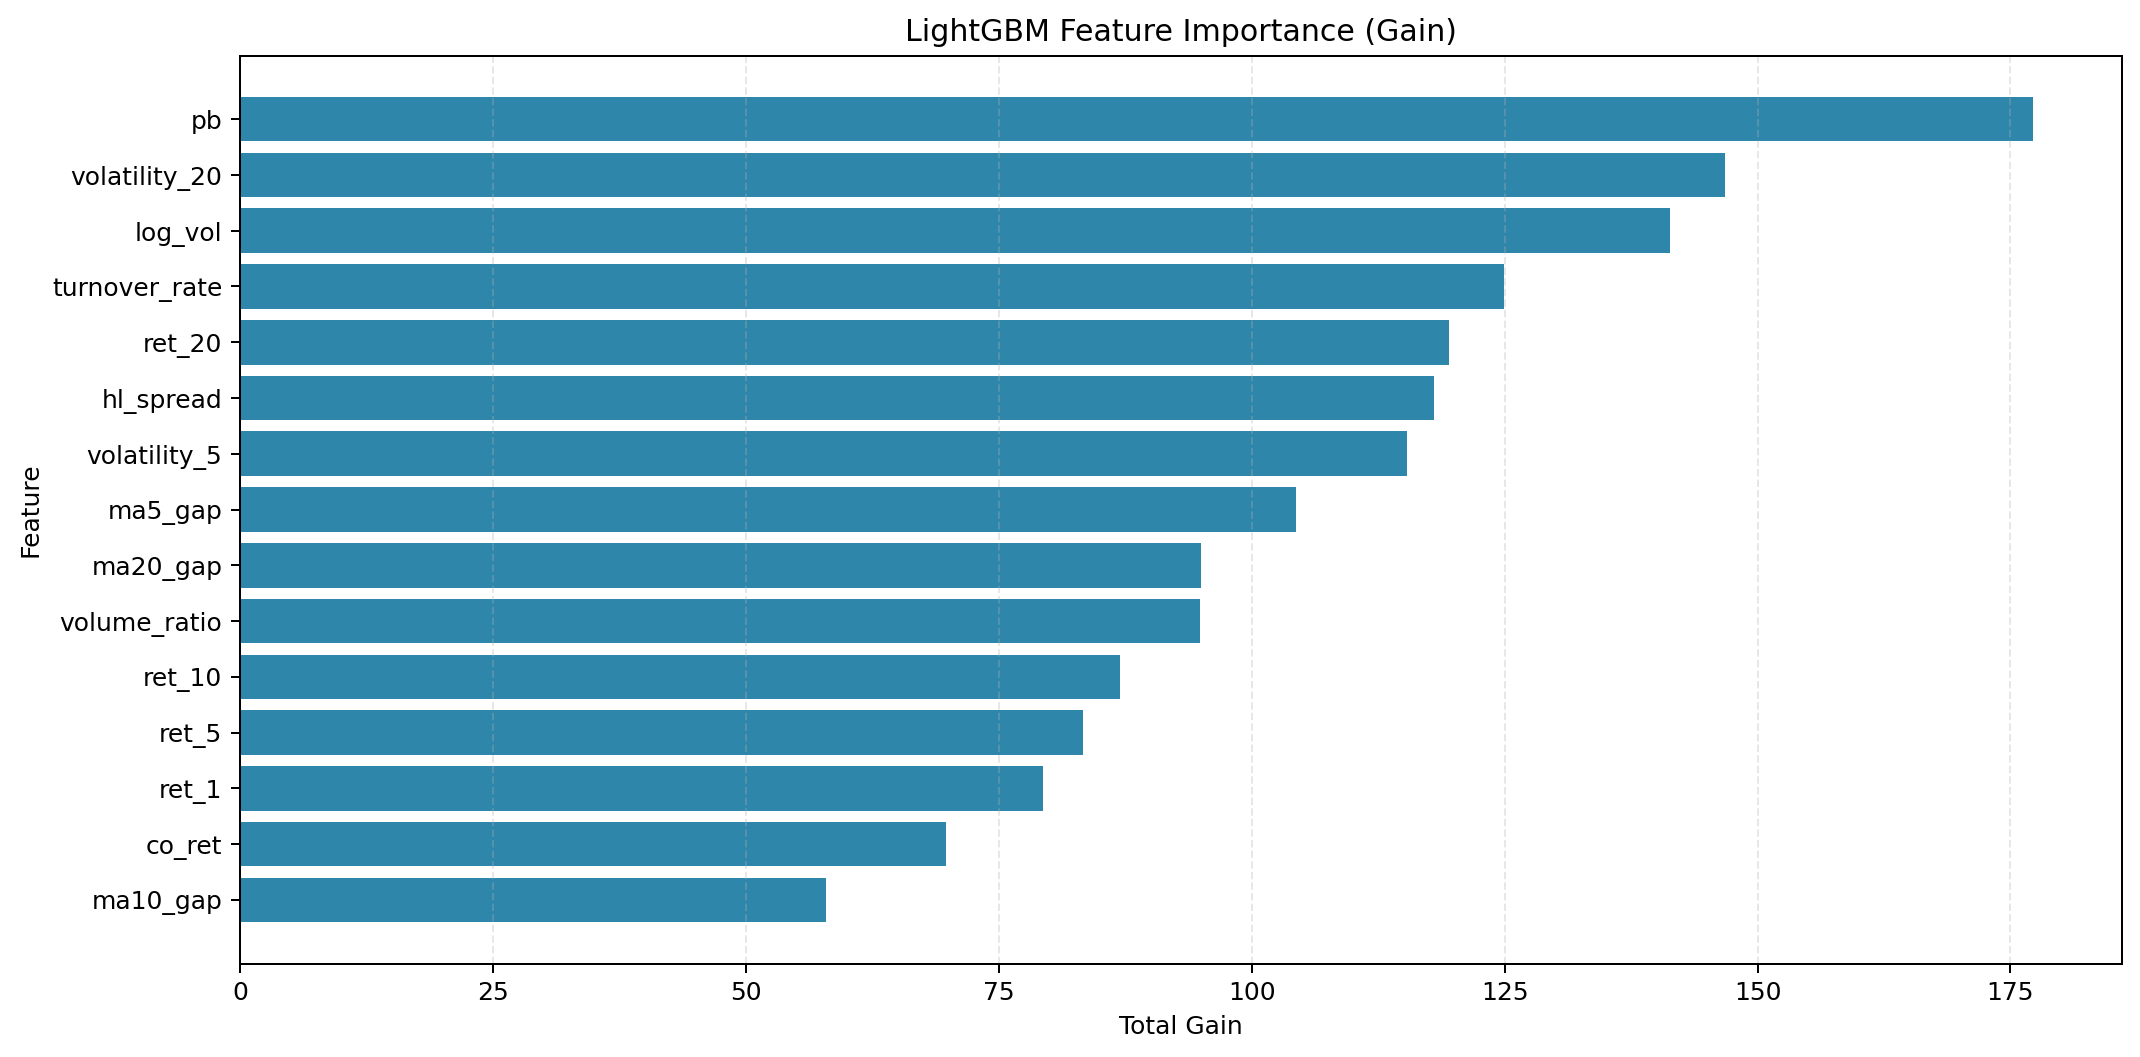
\includegraphics[width=0.95\textwidth]{experiment/feature_importance_gain_price_only.png}
\caption{Feature importance (by gain) for LightGBM trained on price factors only. Price-based features dominate, with \texttt{pb}, \texttt{volatility\_20}, and \texttt{log\_vol} ranking in the top 3.}
\label{fig:importance-price-only}
\end{figure}

\begin{figure}[htbp]
\centering
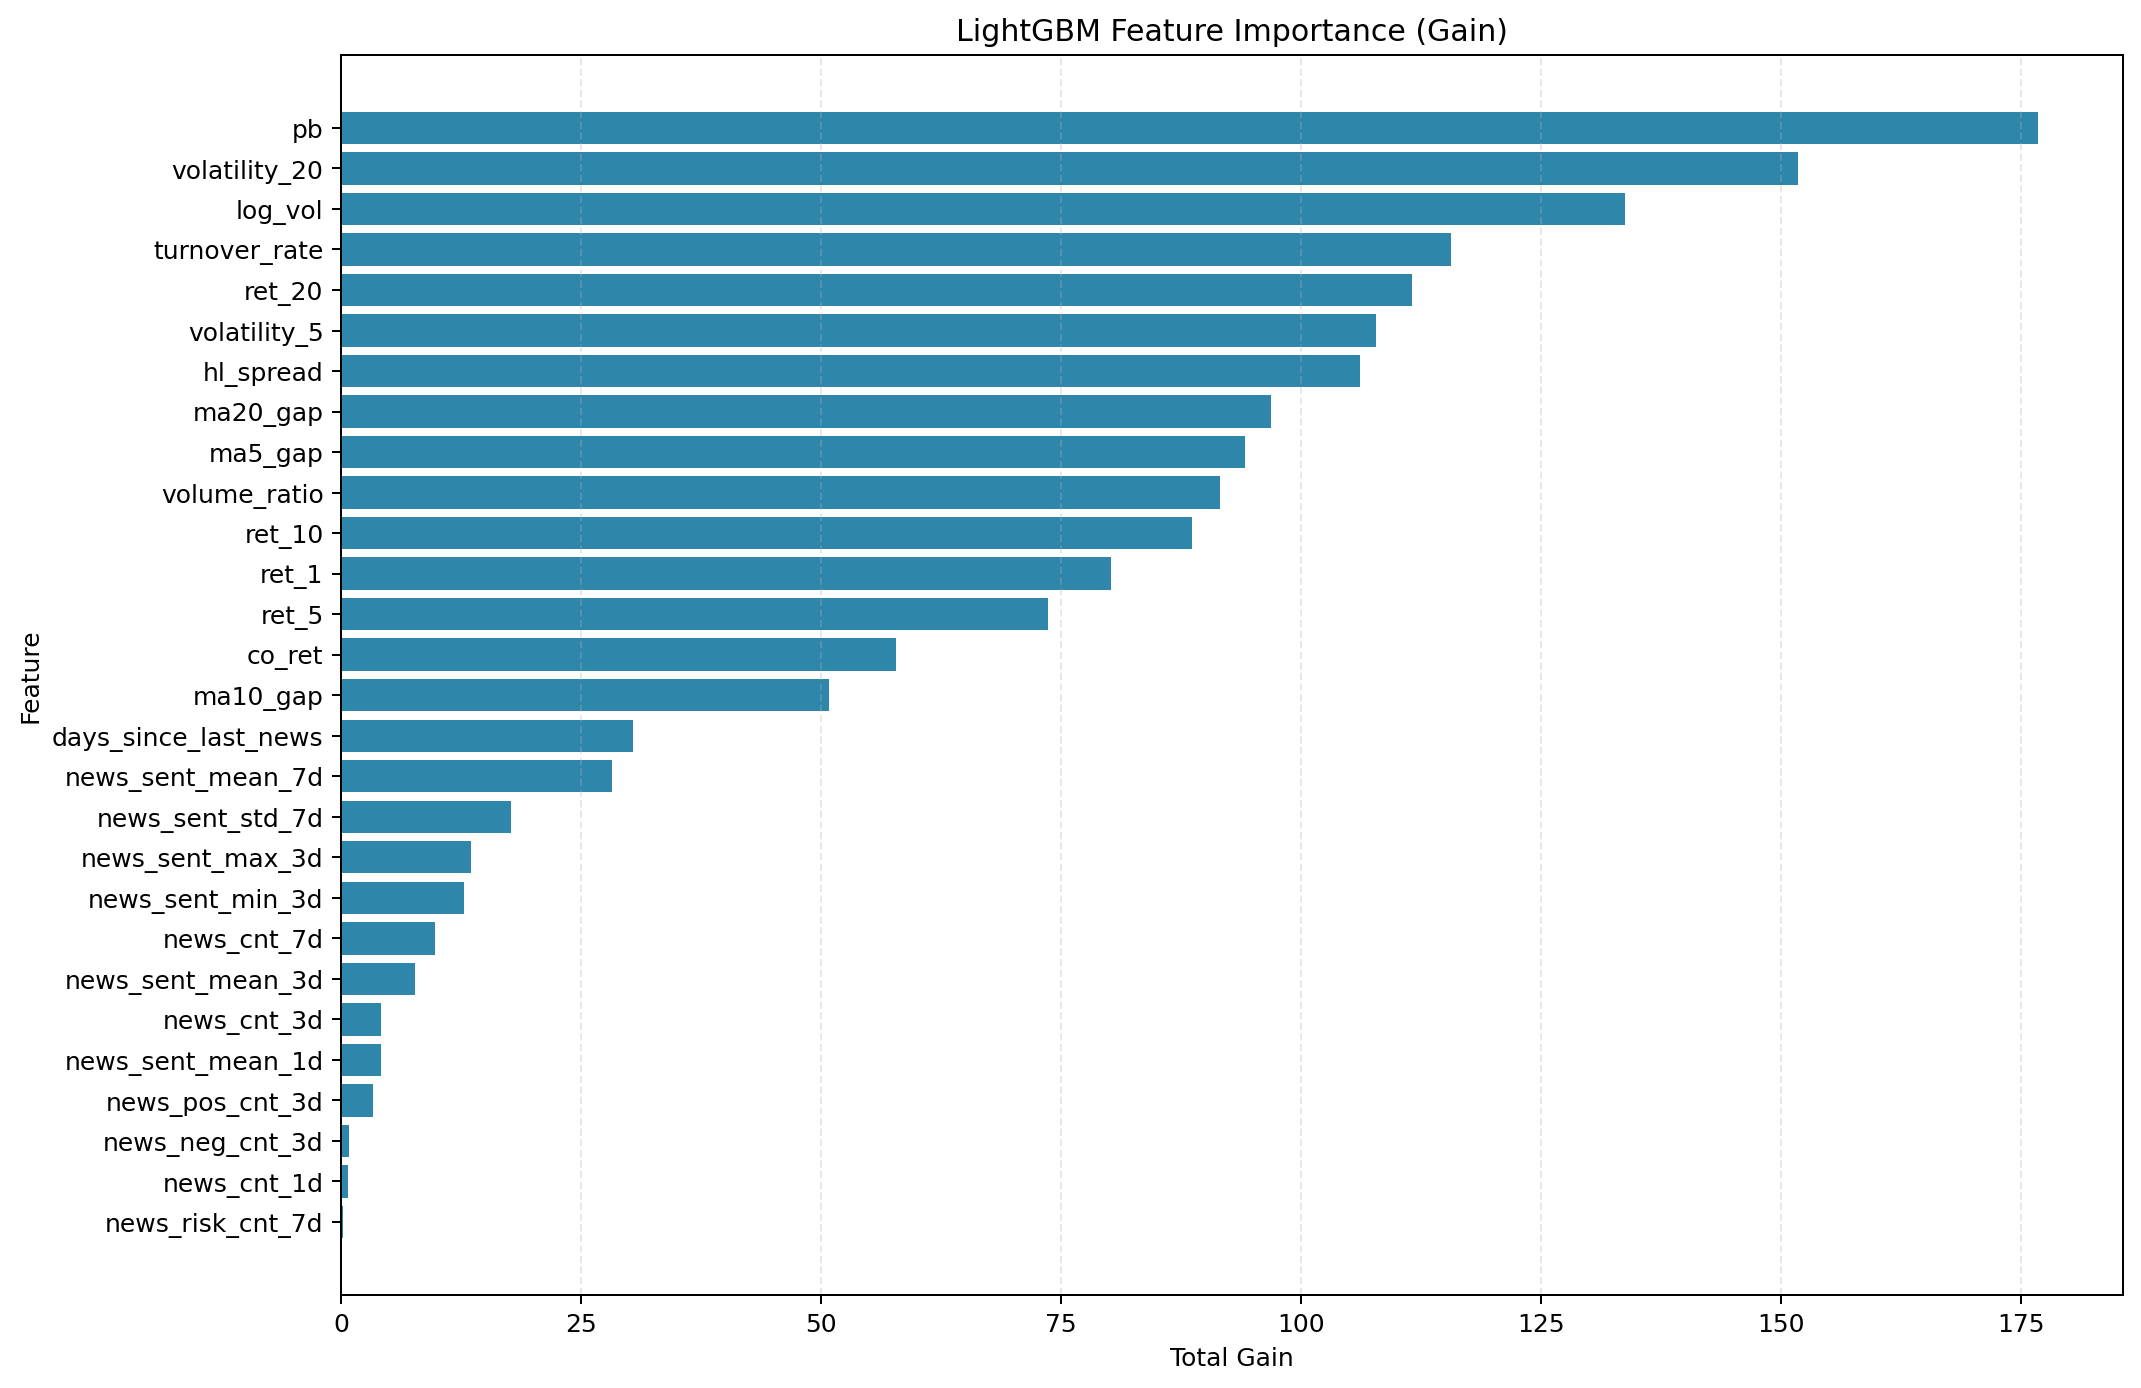
\includegraphics[width=0.95\textwidth]{experiment/feature_importance_gain_price_and_news.png}
\caption{Feature importance (by gain) for LightGBM trained on price and news factors. Price features remain dominant, but news-based features now appear in the ranking, with sentiment-related features (e.g., \texttt{news\_sent\_mean\_7d}) ranking higher than frequency-based features. The highest-ranked news feature (\texttt{days\_since\_last\_news}) is ranked 16th overall.}
\label{fig:importance-news-augmented}
\end{figure}

Key observations from the feature importance analysis are:

\begin{itemize}
\item \textbf{Price factors remain dominant.} In both the price-only and news-augmented models, price-based features occupy the top 15 rankings. \texttt{pb}, \texttt{volatility\_20}, and \texttt{log\_vol} are consistently ranked in the top 3, confirming that price factors capture the primary predictive signal.

\item \textbf{News features are actively utilized.} News features appear among the ranked features in the news-augmented model, indicating that LightGBM actively leverages news information during training. Notably, sentiment-based features (\texttt{news\_sent\_mean\_7d}, \texttt{news\_sent\_std\_7d}, \texttt{news\_sent\_max\_3d}) rank higher in importance than frequency-based features (\texttt{news\_cnt\_*}), suggesting that the \textbf{tone and distribution of news matter more than volume alone}.

\item \textbf{News serves as a complementary signal.} The improvement in top-$k$ selection without a corresponding improvement in overall IC confirms that news features provide targeted filtering rather than systematic ranking improvement. This aligns with the interpretation that news identifies regime shifts or high-impact events that affect subsets of stocks.

\end{itemize}

\subsection{Discussion and Interpretation}

The differential impact of news across model architectures reveals fundamental insights into how different models handle event-driven information:

\begin{enumerate}
\item \textbf{Event-driven vs.\ time-series representation.} News features are inherently event-driven and sparse, fundamentally different from traditional time-series features. Tree-based models excel at capturing such sparse and non-linear signals through their split-based decision structure, while sequential models struggle because they rely on smooth temporal dependencies.

\item \textbf{Model architecture determines information utilization.} The contrasting results for tree models (improvement) and GRU (degradation) demonstrate that model architecture is critical for leveraging multimodal information. Tree models treat each feature independently and can ignore noise, whereas RNNs attempt to learn temporal correlations among all inputs, making them sensitive to sparse noise.

\item \textbf{Implication for graph-based modeling.} These findings suggest that news information is better modeled through \textbf{relational and event-driven dependencies rather than as a time series}. This motivates the use of graph neural networks, which can explicitly represent event propagation, cross-stock relationships, and temporal event sequences in a structured manner.

\end{enumerate}

\subsection{Baseline Selection}

Compared with price-only baselines, incorporating news yields consistent but modest improvements in tree models, while degrading GRU performance. Therefore, under the current non-graph setting, \textbf{LightGBM + price + news} is selected as the strongest non-graph multimodal baseline for subsequent comparison with graph-based approaches.

\begin{table}[htbp]
\centering
\caption{News-enhanced model performance on 2025 test set}
\label{tab:news-test-results}
\begin{tabular}{lcccc}
\hline
Model & Test IC & Test RankIC & Top30 Sharpe & Top50 Sharpe \\
\hline
XGBoost + News & 0.04874212 & 0.01384341 & 4.61825196 & 4.54984642 \\
LightGBM + News & \textbf{0.05116316} & 0.01545951 & \textbf{4.84635056} & \textbf{4.72459068} \\
GRU + News & 0.02691771 & 0.01575878 & 3.29921022 & 2.99269869 \\
\hline
\end{tabular}
\end{table}

\begin{table}[htbp]
\centering
\caption{Change from price-only to price+news on test set}
\label{tab:news-vs-price-delta}
\begin{tabular}{lccc}
\hline
Model & $\Delta$ Test IC & $\Delta$ Top30 Sharpe & $\Delta$ Top50 Sharpe \\
\hline
XGBoost & +0.00008107 & +0.39023861 & +0.09317383 \\
LightGBM & +0.00142095 & +0.62126981 & +0.37211872 \\
GRU & -0.02468536 & -0.71000960 & -0.60178435 \\
\hline
\end{tabular}
\end{table}

\section{Effect of Policy Features}

\subsection{Two Policy Feature Construction Methods}

To further incorporate macro policy information, we implemented two different policy feature pipelines and compared them under the same LightGBM setup (train 2019--2023, validation 2024, test 2025).

\paragraph{Method A: Market-level policy aggregation}
In the first method, all policy documents are aggregated at the market level by date, without sector differentiation. Daily policy count and sentiment are rolled into 7-day and 30-day windows, producing:
\texttt{policy\_cnt\_7d}, \texttt{policy\_cnt\_30d}, \texttt{policy\_support\_score\_7d}, \texttt{policy\_support\_score\_30d}, and \texttt{days\_since\_last\_policy}.
These features are then merged to all stocks on the same date.

\paragraph{Method B: Sector-aware policy aggregation}
In the second method, each stock is mapped to a sector and policy records contain sector relevance weights. For a policy sentiment score $s$, sector weight $w$, and global policy sentiment mean $\mu$, we compute a sector-adjusted score
\[
s_{\text{adj}} = \mu + (s - \mu) \cdot w.
\]
Only positive sector-match weights are kept as effective signals. Then for each stock, sector-level policy signals are rolled over time into:
\texttt{policy\_7d}, \texttt{policy\_30d}, \texttt{policy\_cnt\_7d}, and \texttt{days\_since\_last\_policy}.
All policy features are shifted by one day to avoid leakage.
This design aims to convert policy information from a market-wide signal into a stock-specific sector-aware signal.

\subsection{Comparison Between the Two Policy Methods}

Table~\ref{tab:policy-method-comparison} reports the direct comparison. The old market-level method shows high in-sample fit but fails to generalize (negative test IC). The sector-aware method substantially improves robustness: validation IC remains modest, but test IC returns to a clear positive value and Top-$k$ Sharpe is strong.

\begin{table}[htbp]
\centering
\caption{Comparison of two policy feature construction methods (LightGBM + price + news + policy)}
\label{tab:policy-method-comparison}
\begin{tabular}{lcccc}
\hline
Method & Test IC & Test RankIC & Top30 Sharpe & Top50 Sharpe \\
\hline
Market-level policy aggregation (Method A) & -0.03577257 & -0.03729665 & 3.73783433 & 4.24234969 \\
Sector-aware policy aggregation (Method B) & 0.04646233 & 0.01076620 & 4.81798179 & 4.86964543 \\
\hline
\end{tabular}
\end{table}

This confirms that the sector-aware design is a meaningful correction over the earlier policy formulation. In other words, policy features are no longer ``dangerous'' enough to collapse out-of-sample IC, but become a controllable auxiliary signal.

\subsection{Feature Importance Comparison for Two Policy Methods}

We further compare feature importance distributions of the two policy methods in Figures~\ref{fig:importance-policy-method-a} and~\ref{fig:importance-policy-method-b}.

\begin{figure}[htbp]
\centering
\includegraphics[width=0.95\textwidth]{experiment/feature_importance_gain_policy.png}
\caption{Feature importance (gain) under Method A (market-level policy aggregation). Policy features dominate the top ranks, and this version exhibits poor out-of-sample IC.}
\label{fig:importance-policy-method-a}
\end{figure}

\begin{figure}[htbp]
\centering
\includegraphics[width=0.95\textwidth]{experiment/feature_importance_gain_sector.png}
\caption{Feature importance (gain) under Method B (sector-aware policy aggregation). Policy features are still strong, but the model generalization is substantially improved.}
\label{fig:importance-policy-method-b}
\end{figure}

Under Method B, policy features still occupy the top positions (e.g., \texttt{policy\_30d}, \texttt{days\_since\_last\_policy}, \texttt{policy\_7d}), indicating that policy signal remains very influential. This explains why the method improves Top-$k$ selection but does not consistently improve full cross-sectional ranking stability year by year.

\subsection{Comparison with the Best Previous Baseline}

Although Method B is a clear improvement over Method A, it does not consistently outperform the strongest previous baseline (LightGBM + price + news, without sector-policy features) in overall ranking quality:

\begin{itemize}
\item Best previous baseline (price + news): Test IC $\approx 0.0512$, Top30 Sharpe $\approx 4.846$, Top50 Sharpe $\approx 4.725$
\item Sector-policy version (price + news + sector-policy): Test IC $=0.0465$, Top30 Sharpe $=4.818$, Top50 Sharpe $=4.870$
\end{itemize}

Therefore, policy currently behaves more like a \textbf{top-$k$ filtering enhancer} than a robust \textbf{global ranking enhancer}. It can improve head-portfolio selection in some periods, but does not yet provide a stable IC uplift over the strongest price+news baseline.
This suggests that policy signals may be more regime-dependent and sparse than price and news features, which limits their ability to provide stable full-universe ranking improvement.

\subsection{Conclusion for Policy Experiments}

The policy experiment can be summarized as:
\begin{itemize}
\item Method A (market-level policy) is overfitted and unstable out-of-sample.
\item Method B (sector-aware policy) successfully fixes the major failure mode and restores positive test IC.
\item However, policy features are still relatively dominant and temporally unstable; gains are stronger in Top-$k$ selection than in full-universe ranking.
\item For the current report, \textbf{LightGBM + price + news} remains the strongest and most stable non-graph baseline, while \textbf{sector-aware policy} is a promising but not yet consistently superior extension.
\end{itemize}

\section{First GNN Baseline: GCN with Industry Graph}

After establishing strong non-graph baselines, we begin to test graph neural networks. This is the first GNN in the project, and it is intentionally price-only: there are no news or policy features in this version. The objective is to isolate the contribution of graph structure itself.

\subsection{How the Graph Is Built}

The graph is constructed from the industry mapping file \texttt{zz500\_stock\_sector\_map.txt}. Each stock is treated as a node, and an edge is created between two stocks if they belong to the same sector. In practice, this produces an industry adjacency matrix where stocks within the same sector are fully connected, including self-connections on the diagonal.

This graph is then converted into \texttt{edge\_index} for PyTorch Geometric, so that the GCN can perform message passing over industry-linked stocks.

\subsection{How the Dataset Is Built}

To separate dataset construction from model training, we first generate a graph dataset on disk. The pipeline reads the monthly parquet files under \texttt{dataset\_by\_month}, fixes a global stock order from the sector map, and then creates one daily snapshot per trading day.

Each snapshot contains:
\begin{itemize}
\item \texttt{x}: node feature matrix of size $N \times 15$
\item \texttt{y}: future return target
\item \texttt{mask}: valid-label indicator for each stock
\item \texttt{trade\_date}: the corresponding trading date
\end{itemize}

The split remains strictly chronological:
\begin{itemize}
\item Train: 2019--2023
\item Validation: 2024
\item Test: 2025
\end{itemize}

This ensures that the graph experiment follows exactly the same no-leakage protocol as the LightGBM and GRU baselines.

\subsection{GCN Design and Hyperparameters}

The model is a simple two-layer GCN:
\begin{itemize}
\item \texttt{GCNConv(15, 32)}
\item ReLU activation
\item Dropout disabled in the final stable run (\texttt{dropout = 0.0})
\item \texttt{GCNConv(32, 1)}
\end{itemize}

The final training configuration is:
\begin{itemize}
\item learning rate: \texttt{0.001}
\item weight decay: \texttt{1e-4}
\item early stopping patience: \texttt{20}
\item device: CUDA-only
\item best checkpoint selected by validation IC
\end{itemize}

We explicitly monitor validation IC after every epoch and keep the best model state. In our run, the best validation epoch is epoch 36, and the training stops at epoch 56 because validation IC no longer improves.

\subsection{Results}

\textbf{Note on evaluation protocol:} The following results report the best single-run checkpoint selected by validation IC. This differs from the repeated-run aggregated means reported in later sections (Section \\ref{sec:repeated-run-check}). Single-run results are included here to understand early-stage model behavior; fair cross-model comparison uses the repeated-run protocol.

The final GCN result on the 2025 test set is:
\begin{itemize}
\item Validation IC $=0.0692$
\item Test IC $=0.0561$
\item Test Top30 Sharpe $=4.1731$
\item Test Top50 Sharpe $=4.0833$
\end{itemize}

Compared with the price-only LightGBM baseline without news, which gives validation IC $=0.0529$, test IC $=0.0497$, Top30 Sharpe $=4.2251$, and Top50 Sharpe $=4.3525$, the GCN shows a clear improvement in IC-based ranking quality:
\begin{itemize}
\item Test IC: $0.0561 > 0.0497$
\item Validation IC: $0.0692 > 0.0529$
\end{itemize}

This is the key message of the first graph experiment: even without news or policy, the industry graph itself adds predictive value beyond price features. The GCN is therefore learning not only stock-level price patterns, but also the relational structure between stocks within the same sector.

At the same time, the head-portfolio metrics are still slightly weaker than LightGBM in this run:
\begin{itemize}
\item Top30 Sharpe: $4.1731 < 4.2251$
\item Top50 Sharpe: $4.0833 < 4.3525$
\end{itemize}

So the most accurate summary is that GCN improves global cross-sectional ranking quality, while LightGBM remains slightly stronger in some Top-$k$ portfolio metrics. This is still a strong result, because it shows that graph structure can contribute useful information even in a price-only setting.

\subsection{Takeaway}

This experiment gives a clean foundation for later graph-based work. It shows that a simple industry graph is already enough to beat the price-only LightGBM in IC, which justifies moving on to more advanced graph variants such as GAT, or to multimodal graph models that combine price, news, and policy information.

\section{GCN + News: Naive Feature Fusion Experiment}

After the price-only GCN baseline, we directly extend the node feature space by concatenating the 13 daily aggregated news features to the 15 price features, resulting in a 28-dimensional input per stock node. The goal is to test whether a straightforward multimodal fusion strategy can further improve graph-based prediction.

\subsection{Method}

The graph topology is unchanged from the previous GCN experiment: an industry graph built from sector relations, with message passing performed over the same fixed \texttt{edge\_index}. The dataset is rebuilt from the price+news monthly parquet files, and each daily snapshot contains:
\begin{itemize}
\item \texttt{x}: $N \times 28$ node feature matrix (15 price + 13 news)
\item \texttt{y}: \texttt{future\_ret\_5}
\item \texttt{mask}: valid-label indicator
\item \texttt{trade\_date}: snapshot date
\end{itemize}

The chronological split remains unchanged (train 2019--2023, validation 2024, test 2025), ensuring a fair comparison with all previous baselines.

Model and training setup:
\begin{itemize}
\item Architecture: two-layer GCN, \texttt{GCNConv(28, 32)} $\rightarrow$ ReLU $\rightarrow$ \texttt{GCNConv(32, 1)}
\item Optimizer: Adam, learning rate \texttt{0.001}, weight decay \texttt{1e-4}
\item Dropout: \texttt{0.0}
\item Early stopping patience: \texttt{20} (monitored by validation IC)
\item Device: CUDA
\end{itemize}

In this run, early stopping is triggered at epoch 26 (\texttt{early\_stopping\_triggered\_at\_epoch=026}).

\subsection{Results}

\textbf{Note on evaluation protocol:} This result is from a single run with best checkpoint selection by validation IC, consistent with the diagnostic stage before repeated-run aggregation.

\begin{table}[htbp]
\centering
\caption{GCN + news (naive feature fusion) performance}
\label{tab:gcn-news-results}
\begin{tabular}{lccccc}
\hline
Split & IC & RankIC & SignAcc & Sharpe & MSE \\
\hline
Train & 0.02570720 & 0.01694803 & 0.51022165 & -0.01330520 & 0.00493104 \\
Validation & 0.02815299 & 0.03480681 & 0.51884070 & 0.08337738 & 0.00607030 \\
Test & 0.01774965 & -0.01090303 & 0.48513127 & -0.22383365 & 0.00389935 \\
\hline
\end{tabular}
\end{table}

Top-$k$ portfolio metrics are:
\begin{itemize}
\item Train: Top10 IRR $=0.57108011$, Top10 Sharpe $=0.99038085$; Top30 IRR $=1.21270513$, Top30 Sharpe $=1.54181882$; Top50 IRR $=1.41018173$, Top50 Sharpe $=1.72388718$
\item Validation: Top10 IRR $=1.23593125$, Top10 Sharpe $=1.31856354$; Top30 IRR $=1.03630241$, Top30 Sharpe $=1.19862977$; Top50 IRR $=0.51437948$, Top50 Sharpe $=0.88606933$
\item Test: Top10 IRR $=2.79205900$, Top10 Sharpe $=2.55943744$; Top30 IRR $=1.83442621$, Top30 Sharpe $=2.26488221$; Top50 IRR $=1.51323129$, Top50 Sharpe $=2.08909511$
\end{itemize}

The key signal is that test IC and test RankIC are weaker than the price-only GCN baseline, despite adding more information channels.

\subsection{Interpretation and Conclusion}

While news features improve performance in non-graph models, directly incorporating them into GCN leads to performance degradation. This suggests that naive feature fusion under graph propagation may amplify noise and harm cross-sectional ranking. Proper feature scaling and selective aggregation are necessary for effective integration.

In short, naive feature fusion can degrade performance under graph propagation. A plausible reason is that standard GCN performs fixed neighborhood averaging and cannot distinguish which neighbor is more informative under sparse event-driven news shocks.

\subsection{Next Session Direction: Processed/Filtered News + Better Graph Attention}

The next stage should move from raw concatenation to \textbf{processed/filtered news + GCN}: denoising, scaling, or gating news channels before message passing, so that event signals do not dominate or contaminate all neighbors.

At the same time, replacing GCN with GAT is well-motivated. The current bottleneck is that GCN cannot distinguish ``which neighbor matters more,'' while GAT can learn attention weights and adaptively focus on informative neighbors. Therefore, \textbf{processed/filtered news + GAT} is a strong candidate for the next iteration.

\section{Processed/Filtered News Session: From Raw Signals to Compact Graph Inputs}

This section reports the next stage after naive news fusion. We first redesign the news pipeline in \texttt{build\_feature\_news\_graph.py}, then compare two graph-input settings under the same GCN framework:
\begin{itemize}
\item \textbf{27-feature setting}: 15 price + 12 processed news features
\item \textbf{21-feature setting}: 15 price + 6 compact news features
\end{itemize}

\subsection{What Changed in \texttt{build\_feature\_news\_graph.py}}

Compared with the earlier raw-news style aggregation, the new processing introduces three key changes designed for graph stability:

\begin{enumerate}
\item \textbf{Sentiment mean is replaced by sentiment deviation.}
Instead of directly using \texttt{news\_sent\_mean\_*} with a fixed default baseline, we use
\[
\texttt{news\_sent\_dev} = \texttt{sentiment\_mean} - \mu_{\text{news}}
\]
where $\mu_{\text{news}} = 0.732936$. Missing-news cases are set to zero deviation.

\item \textbf{Count channels are compressed and gated.}
Raw counts are replaced by \texttt{log1p} versions (e.g., \texttt{news\_cnt\_7d\_log}), and explicit event indicators (\texttt{has\_news\_*}) are added.

\item \textbf{Recency is transformed into freshness.}
Instead of using extreme raw gap values, recency is converted to
\[
\texttt{news\_freshness} = \exp(-\texttt{days}/7).
\]
In the compact graph builder, \texttt{news\_freshness} is additionally forced to zero when \texttt{has\_news\_7d}=0, and \texttt{news\_sent\_std\_7d} is clipped at 0.2.
\end{enumerate}

All news features are still shifted by one trading day to avoid leakage.

\subsection{Experiment A: Processed News with 27 Features (15+12)}

\textbf{Evaluation protocol:} This section reports single-run best checkpoints selected by validation IC. These diagnostic results precede the repeated-run aggregation used in the final validation section.

This setting uses the full processed news feature set:
\begin{itemize}
\item \texttt{has\_news\_1d}, \texttt{has\_news\_3d}, \texttt{has\_news\_7d}
\item \texttt{news\_cnt\_1d\_log}, \texttt{news\_cnt\_3d\_log}, \texttt{news\_cnt\_7d\_log}
\item \texttt{news\_sent\_dev\_1d}, \texttt{news\_sent\_dev\_3d}, \texttt{news\_sent\_dev\_7d}
\item \texttt{news\_sent\_std\_7d}, \texttt{news\_risk\_cnt\_7d\_log}, \texttt{news\_freshness}
\end{itemize}

Main results:
\begin{itemize}
\item Best validation IC: $0.05982203$ (epoch 7)
\item Test IC: $0.02790876$
\item Test RankIC: $0.04116817$
\item Test Top30 Sharpe: $2.31734319$
\item Test Top50 Sharpe: $2.38834289$
\end{itemize}

\subsection{Experiment B: Compact Processed News with 21 Features (15+6)}

This setting keeps only six news channels:
\begin{align*}
\{&\texttt{has\_news\_7d},\ \texttt{news\_cnt\_7d\_log},\ \texttt{news\_sent\_dev\_7d},\\
&\texttt{news\_sent\_std\_7d},\ \texttt{news\_risk\_cnt\_7d\_log},\ \texttt{news\_freshness}\}
\end{align*}

Main results:
\begin{itemize}
\item Best validation IC: $0.06348345$ (epoch 19)
\item Test IC: $0.04239240$
\item Test RankIC: $0.03813298$
\item Test Top30 Sharpe: $1.96451284$
\item Test Top50 Sharpe: $2.24241265$
\end{itemize}

\begin{table}[htbp]
\centering
\caption{Processed-news GCN comparison: 27 vs 21 features}
\label{tab:gcn-processed-news-27-vs-21}
\begin{tabular}{lccccc}
\hline
Setting & Best Val IC & Test IC & Test RankIC & Top30 Sharpe & Top50 Sharpe \\
\hline
GCN + 27 features (15+12) & 0.05982203 & 0.02790876 & 0.04116817 & 2.31734319 & 2.38834289 \\
GCN + 21 features (15+6) & \textbf{0.06348345} & \textbf{0.04239240} & 0.03813298 & 1.96451284 & 2.24241265 \\
\hline
\end{tabular}
\end{table}

\subsection{What This Means}

Two conclusions are clear.

\paragraph{(1) Compact processed news is better than noisier news formulations.}
Relative to the earlier raw-news fusion results (which showed weaker test IC and even negative RankIC in this report), the processed/compact pipeline improves stability: test IC returns to a positive and clearly higher level, and training dynamics are more controlled.

\paragraph{(2) News still does not improve GCN over price-only.}
Even after substantial feature cleaning, the best compact setting (test IC $=0.04239240$) remains below the price-only GCN baseline reported earlier (test IC $=0.0561$). Therefore, the issue is no longer just ``raw news is noisy.'' A deeper issue is the \textbf{naive way news is injected into node features and then propagated by GCN}.

\subsection{Why Compact News Can Still Hurt Under GCN}

\begin{enumerate}
\item \textbf{News is event-driven, not a stable structural state.}
Price factors (return, volatility, valuation, liquidity) are relatively persistent node-state variables. News is sparse and shock-like. Treating both as homogeneous node attributes is not ideal.

\item \textbf{Industry message passing is naturally aligned with price, not always with news.}
Industry co-movement is plausible for price factors, but firm-specific news is often idiosyncratic. Uniform propagation can spread local events to weakly related neighbors.

\item \textbf{Standard GCN has limited selectivity.}
Vanilla GCN aggregates neighbors with fixed normalization and no feature-level gating. It cannot explicitly decide which event signal should be propagated and to whom.
\end{enumerate}

\subsection{Research Implication and Next Architecture}

This result chain is important:
\begin{itemize}
\item News helps tree models in non-graph settings.
\item Price-only GCN is strong.
\item GCN + raw news degrades.
\item GCN + compact news degrades less, but still does not beat price-only GCN.
\end{itemize}

So the practical next step is \textbf{not} ``add more news channels into the same GCN input,'' but a modality-aware architecture:
\begin{itemize}
\item \textbf{Price branch:} price features go through GCN to model cross-stock relational structure.
\item \textbf{News branch:} compact news features go through an MLP (or gated MLP) as event encoder.
\item \textbf{Fusion:} late fusion (concatenation + MLP head, or gated additive fusion) combines price-graph embedding and news embedding for final return prediction.
\end{itemize}

This design preserves the advantage of graph propagation for structural price signals, while avoiding indiscriminate diffusion of sparse event shocks.

\subsection{Residual News Fusion Ablation and Interim Summary}

To further test whether compact news signals can be injected more safely, we evaluate a residual fusion design on top of the 21-feature setting (15 price + 6 news):
\[
\hat{y} = \hat{y}_{\text{price}} + \alpha \cdot \Delta_{\text{news}},
\]
where the price branch is a GCN predictor and the news branch is a small MLP that outputs a scalar correction term. We test three residual weights: $\alpha \in \{0.05, 0.1, 0.2\}$.

Compared with the earlier concat-fusion model, residual fusion is clearly more stable during training: predictions do not collapse to a near-constant output as quickly, and validation IC remains meaningful across epochs. However, the key question is whether residual news fusion can beat the strongest graph baseline, i.e., price-only GCN.

\begin{table}[htbp]
\centering
\caption{Price-only GCN vs residual news fusion (2025 test set)}
\label{tab:gcn-residual-news-vs-price}
\begin{tabular}{lcccc}
\hline
Model & Val IC & Test IC & Test RankIC & Top50 Sharpe \\
\hline
GCN price-only & \textbf{0.0692} & \textbf{0.0561} & \textbf{0.0470} & \textbf{4.0833} \\
Residual $\alpha=0.10$ & 0.0676 & 0.0391 & 0.0363 & 2.0537 \\
Residual $\alpha=0.20$ & 0.0678 & 0.0455 & 0.0374 & 1.8038 \\
Residual $\alpha=0.05$ & 0.0603 & 0.0333 & 0.0470 & 2.7287 \\
\hline
\end{tabular}
\end{table}

The residual ablation leads to three final findings:
\begin{itemize}
\item \textbf{Residual fusion is more stable than concat fusion.} Adding news as a constrained correction term is better behaved than direct feature concatenation.
\item \textbf{The best residual setting is $\alpha=0.2$ by Test IC, but it still underperforms price-only GCN.} The best residual Test IC is $0.0455$, still below $0.0561$ from price-only GCN.
\item \textbf{News does not provide positive net gain for GCN on \texttt{future\_ret\_5} in this setup.} Under both concat and residual fusion, news tends to dilute the strong structural price signal already captured by the graph branch.
\end{itemize}

\section{Data and Graph}

This section now shifts focus to data and graph design changes. The goal is to test whether better data representation and relation graphs can improve robustness and generalization beyond simple architecture substitution.

\subsection{GAT Experiments: Single-Run Diagnostic}

Based on the previous experiments, moving from GCN to GAT is a natural next step. The earlier results show that (i) price-only graph modeling is effective, (ii) naive and even processed news fusion can still degrade graph performance, and (iii) fixed neighborhood averaging in vanilla GCN has limited selectivity for sparse, event-driven signals. Therefore, we introduce GAT to test whether \textbf{adaptive neighbor weighting} can better utilize relational information than fixed normalization.

\textbf{Important note on evaluation protocol:} The GAT experiments in this section use a single-run best-epoch protocol to diagnose model behavior under different loss functions. This differs from the repeated-run aggregation used later in Section \ref{sec:repeated-run-check}. These results are intended as a diagnostic stage to understand failure modes, not a final cross-architecture comparison. Fair horizontal comparison across all four models will be performed in the subsequent repeated-run section.

In this section, we first report a clean \textbf{price-only} GAT study as the first subsection, then compare three training objectives under identical architecture and data split.

\subsection{Price-Only ResidualGAT: Controlled Loss Study}

To ensure fair comparison, we keep the same data protocol as previous graph experiments:
\begin{itemize}
\item Train period: 2019--2023
\item Validation period: 2024
\item Test period: 2025
\item Target: \texttt{future\_ret\_5}
\item Input features: 15 price factors
\item Graph: industry-relation graph with fixed \texttt{edge\_index}
\end{itemize}

All runs use identical optimization settings unless otherwise noted: learning rate $=0.0005$, weight decay $=10^{-4}$, dropout $=0.0$, early stopping patience $=20$, hidden dimension $=32$, and attention heads $=4$.

\subsubsection{ResidualGAT Architecture Design}

The model is a two-layer residual GAT with normalization and a lightweight prediction head:
\begin{itemize}
\item Input projection: \texttt{Linear(15, 32)}
\item Layer 1: \texttt{GATConv(32, 8, heads=4, concat=True)}
\item Residual normalization: \texttt{LayerNorm(h + h1)}
\item Layer 2: \texttt{GATConv(32, 8, heads=4, concat=True)}
\item Residual normalization: \texttt{LayerNorm(h + h2)}
\item Prediction head: \texttt{Linear(32,16) \rightarrow ReLU \rightarrow Linear(16,1)}
\end{itemize}

This design preserves stable training through residual connections while allowing node-wise adaptive neighbor weighting through attention heads.

\subsubsection{Three Controlled Loss-Function Experiments}

We run three experiments where \textbf{only the training objective is changed}:

\paragraph{Experiment 1: MSE loss}
\[
\mathcal{L}_{\mathrm{mse}}=\frac{1}{n}\sum_{i=1}^n(\hat{y}_i-y_i)^2.
\]

\paragraph{Experiment 2: IC loss}
\[
\mathcal{L}_{\mathrm{ic}}=-\mathrm{Corr}(\hat{y},y).
\]

\paragraph{Experiment 3: Mixed IC+MSE loss}
\[
\mathcal{L}_{\mathrm{mix}}=\alpha\,\mathcal{L}_{\mathrm{mse}}+\beta\,\mathcal{L}_{\mathrm{ic}},
\quad \alpha=0.2,\ \beta=0.8.
\]

The motivation is straightforward: MSE favors pointwise fit, IC favors cross-sectional ranking, and mixed loss aims to balance both objectives.

\subsubsection{Result Comparison}

\begin{table}[htbp]
\centering
\caption{ResidualGAT price-only: comparison across three loss functions}
\label{tab:residualgat-loss-comparison}
\begin{tabular}{lcccccc}
\hline
Loss & Best Val IC & Best Epoch & Test IC & Test RankIC & Top10 Sharpe & Test MSE \\
\hline
MSE & 0.02831852 & 11 & \textbf{0.02379200} & 0.01326577 & 1.75947725 & \textbf{0.00338399} \\
IC & \textbf{0.04708240} & 4 & 0.00982684 & 0.01687255 & \textbf{5.28420457} & 0.02528161 \\
Mixed IC+MSE & 0.04637430 & 6 & 0.01898695 & \textbf{0.02092624} & 4.31120881 & 0.00643173 \\
\hline
\end{tabular}
\end{table}

\subsubsection{Discussion}

The above results indicate that the current ResidualGAT setting is still unsatisfactory for robust market-wide ranking. 

\textbf{Note on evaluation fairness:} The comparison below uses \textbf{different evaluation protocols} for diagnostic purposes: GAT results are single-run best checkpoints with price-only graph, while the GCN baseline (shown here for context) is a repeated-run mean from the news graph. This is intentionally asymmetric to show diagnostic insights, not a final horizontal comparison. Proper cross-model evaluation under identical protocols will be shown in the repeated-run check section.

The diagnostic comparison is shown below.

\begin{table}[htbp]
\centering
\caption{Diagnostic comparison: ResidualGAT single-run losses vs GCN repeated-run reference}
\label{tab:gat-vs-gcn-key-comparison}
\begin{tabular}{lccc}
\hline
Model & Val IC & Test IC & Test RankIC \\
\hline
GAT + MSE & 0.0283 & 0.0238 & 0.0133 \\
GAT + mixed IC/MSE & 0.0464 & 0.0190 & 0.0209 \\
GAT + IC & 0.0471 & 0.0098 & 0.0169 \\
GCN + news graph (repeated-run mean) & \textbf{0.0673} & \textbf{0.0319} & \textbf{0.0343} \\
\hline
\end{tabular}
\end{table}

The conclusion from this diagnostic comparison is direct: \textbf{GAT does not outperform GCN in the current single-run setting}. Although IC-oriented objectives raise validation IC for GAT, test generalization is weaker, suggesting overfitting to the 2024 validation regime. Note: This conclusion is based on single-run best checkpoints and should not be directly compared to the repeated-run aggregated results shown later.

Two training phenomena are particularly important for explaining why GAT underperforms:
\begin{itemize}
\item \textbf{MSE-version output collapse.} In the MSE run, validation \texttt{pred\_std} rapidly approaches zero, meaning the model degenerates toward an almost constant predictor. This explains why test IC and RankIC remain low even when numerical MSE appears small.
\item \textbf{IC-version scale drift.} In the pure IC run, validation \texttt{pred\_mean}/\texttt{pred\_std}/\texttt{pred\_abs\_max} become large and unstable, while MSE remains very high. This is expected because IC loss is scale-invariant and does not penalize output magnitude, so the model can amplify scores without improving out-of-sample ranking quality.
\item \textbf{Mixed loss partially alleviates but does not solve the issue.} Mixed IC+MSE improves the trade-off and gives the best GAT test RankIC among the three GAT losses, but it still remains below the GCN repeated-run baseline.
\end{itemize}

\subsubsection{Conclusion}

This controlled study shows that, under identical data split and architecture scale, \textbf{the current GAT configuration has not yet learned stable full-market ranking}. The practical conclusion is:
\begin{itemize}
\item GAT does not exceed the GCN baseline.
\item IC-style objectives can improve validation IC but may hurt test generalization.
\item The observed failure modes (MSE-collapse and IC-scale-drift) indicate that objective design and score calibration are the central bottlenecks for this GAT version.
\end{itemize}

Therefore, this GAT result should be treated as a diagnostic stage rather than a final replacement of GCN, and subsequent work should focus on improving ranking stability and cross-period generalization before claiming architecture superiority.

\section{Repeated-Run Check}\label{sec:repeated-run-check}

To consolidate findings across multiple runs and validate robustness, we conduct a unified repeated-run evaluation across four GNN families (GCN, GraphSAGE, APPNP, ResidualGAT) on two graph datasets: (1) \texttt{graph\_dataset} (price-only graph), and (2) \texttt{build\_graph\_news\_graph\_6\_feat} (price + redesigned news graph features). This aggregated comparison uses consistent hyperparameters across all models and reports mean metrics over repeated runs, providing a fair horizontal comparison baseline.

The comparison uses one shared protocol (distinct from the single-run GAT diagnostic in the previous section):
\begin{itemize}
\item Train period: 2019--2023
\item Validation period: 2024
\item Test period: 2025
\item Target: \texttt{future\_ret\_5}
\item Evaluation method: Aggregated mean over repeated runs with identical hyperparameter settings
\item Models compared: GraphSAGE, GCN, APPNP, ResidualGAT
\item Datasets: price-only graph vs redesigned news graph (6 news features)
\item Reporting: All metrics below are means over repeated runs (\textbf{not} single best checkpoints as in earlier diagnostic sections)
\end{itemize}

\paragraph{Interim observation on GCN.}

\begin{table}[htbp]
\centering
\caption{GCN comparison on two graph datasets (test set)}
\label{tab:gcn-final-two-datasets}
\begin{tabular}{lcccc}
\hline
Dataset & Test IC & Test RankIC & Top30 Sharpe & Top50 Sharpe \\
\hline
News graph (6 features) & \textbf{0.0319} & \textbf{0.0343} & \textbf{3.8071} & 3.5712 \\
Price-only graph & 0.0300 & 0.0295 & 3.6584 & \textbf{3.6353} \\
\hline
\end{tabular}
\end{table}

For GCN, adding redesigned news graph features gives a consistent directional gain in ranking quality: Test IC increases from 0.0300 to 0.0319, and Test RankIC increases from 0.0295 to 0.0343.

\paragraph{Cross-model comparison (interim observations).}
\begin{itemize}
\item \textbf{GCN currently gives the strongest IC/RankIC profile in this experiment block.} Under the redesigned news setting, GCN shows the best combined IC/RankIC balance.
\item \textbf{GraphSAGE is strong for top-k portfolio selection, but IC stability is weaker.} On the price-only graph, GraphSAGE reaches very strong Top30/Top50 Sharpe (4.2687/4.3478), but Test IC remains lower (0.0228). With news features, Test IC changes only slightly (0.0232), and Top50 Sharpe drops to 3.9382.
\item \textbf{APPNP benefits slightly from news, but remains mid-tier.} APPNP improves from Test IC 0.0223 to 0.0246 and from Top30 Sharpe 3.2851 to 3.4535 after adding redesigned news features, but it is still weaker than GCN on IC and weaker than GraphSAGE on top-k Sharpe.
\item \textbf{ResidualGAT is weak in the current setup.} Its Test IC decreases from 0.0173 (price-only) to 0.0113 (news graph), suggesting unstable attention learning under noisy financial relations.
\end{itemize}

\paragraph{End of this subsection.}
This block is a small, controlled comparison rather than the final project conclusion. At this stage, GCN with redesigned news features is the most reliable reference setting for subsequent experiments.

